\section{Input Protection, Filtering, and Rectification}
\label{sec:hw-input}

The AC input passes through the connector, fuse, inrush element, varistor, filter, and bridge. The rectified line then supplies the charge pump. The input side includes a capacitor-discharge circuit. The filter connections also carry high-frequency return current from the switching stage and were treated as part of the power loop.

The input fuse is a Littelfuse 04653.15DR rated at \SI{3.15}{\ampere} and \SI{250}{\volt} AC \cite{littelfuse0465315dr}. A Panasonic ERZV07D471 clamps surges \cite{panasonicERZV07D471}. The V1.0 component list specifies a Wurth Elektronik 7448680200 common-mode choke with two \SI{120}{\micro\henry} windings \cite{wurth7448680200}. V1.1 shows a single \SI{100}{\micro\henry} 7447480101 element at L2 instead. This change was made in the drawing; a second filter assembly was not tested.

\begin{figure}[htbp]
\centering
\begin{subfigure}[t]{0.97\textwidth}
\centering
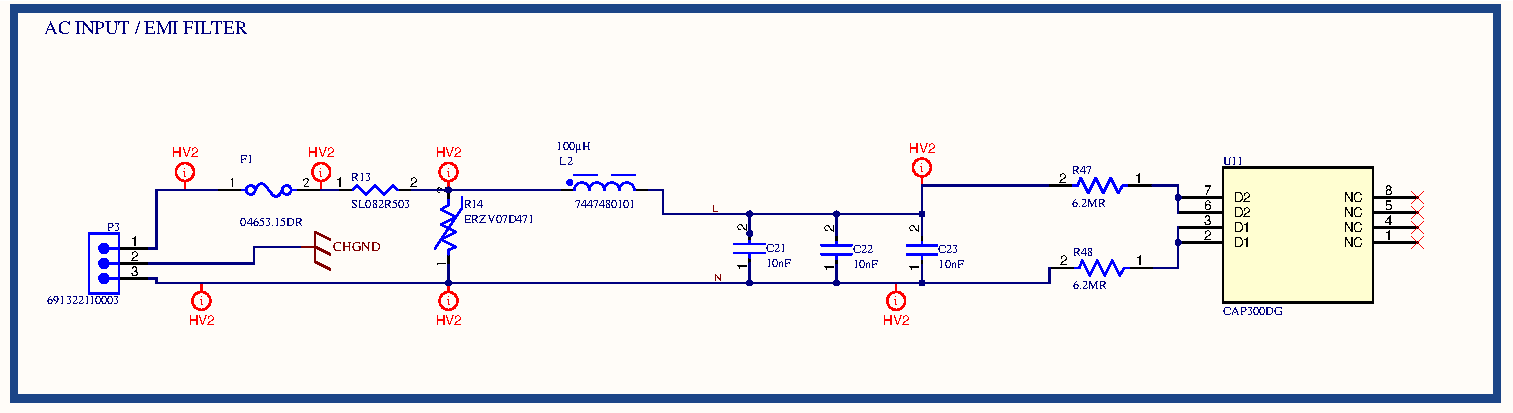
\includegraphics[page=1,width=\textwidth]{Pictures/Thesis/07_Hardware/Rebuilt/schematic_v2_input_excerpt.pdf}
\caption{Input connector, fuse, inrush element, varistor, filter, and discharge circuit.}
\end{subfigure}
\par\medskip
\begin{subfigure}[t]{0.38\textwidth}
\centering
\includegraphics[page=2,width=\textwidth]{Pictures/Thesis/07_Hardware/Rebuilt/schematic_v2_input_excerpt.pdf}
\caption{Bridge rectifier.}
\end{subfigure}
\caption{V2 sheet 3 input filter and full-bridge rectifier.}
\label{fig:hw-input-schematic}
\end{figure}

Bridge commutation, diode capacitance, charge-pump current, and loop inductance couple this path to the half bridge. The assembly's input behavior was assessed from the input-current measurements in Chapter~\ref{ch:results}; measurements on both sides of the installed filter are still needed to determine its noise attenuation.
